\documentclass[journal,12pt,onecolumn]{IEEEtran}

% Import necessary packages
\usepackage{cite}
\usepackage{amsmath,amssymb,amsfonts,amsthm}
\usepackage{algorithmic}
\usepackage{graphicx}
\usepackage{textcomp}
\usepackage{xcolor}
\usepackage{txfonts}
\usepackage{listings}
\usepackage{enumitem}
\usepackage{mathtools}
\usepackage{gensymb}
\usepackage{comment}
\usepackage[breaklinks=true]{hyperref}
\usepackage{tkz-euclide} 
\usepackage{listings}
\usepackage{gvv}                                        
\usepackage[latin1]{inputenc}                                
\usepackage{color}                                            
\usepackage{array}                                            
\usepackage{longtable}                                       
\usepackage{calc}                                             
\usepackage{multirow}                                         
\usepackage{hhline}                                           
\usepackage{ifthen}                                           
\usepackage{lscape}
\usepackage{tabularx}
\usepackage{array}
\usepackage{float}
\usepackage{multicol} % Add the multicol package

% New theorem declarations
\newtheorem{theorem}{Theorem}[section]
\newtheorem{problem}{Problem}
\newtheorem{proposition}{Proposition}[section]
\newtheorem{lemma}{Lemma}[section]
\newtheorem{corollary}[theorem]{Corollary}
\newtheorem{example}{Example}[section]
\newtheorem{definition}[problem]{Definition}

% Custom command definitions
\newcommand{\BEQA}{\begin{eqnarray}}
\newcommand{\EEQA}{\end{eqnarray}}
\newcommand{\define}{\stackrel{\triangle}{=}}

\theoremstyle{remark}
\newtheorem{rem}{Remark}

% Document begins here
\begin{document}
\bibliographystyle{IEEEtran}
\vspace{3cm}

% Title of the document
\title{ASSIGNMENT 3}
\author{EE24BTECH11011 - PRANAY}
\maketitle

\bigskip

% Custom figure and table numbering
\renewcommand{\thefigure}{\theenumi}
\renewcommand{\thetable}{\theenumi}
\begin{enumerate}\setcounter{enumi}{26}
   \item In an experiment, positive and negative values are equally likely to occur. The probability of obtaining at most one negative value in five trials is
   \begin{multicols}{4}
   \begin{enumerate}
       \item $\frac{1}{32}$
       \item $\frac{2}{32}$
       \item $\frac{3}{32}$
       \item $\frac{6}{32}$
   \end{enumerate}
   \end{multicols}
   \item The eigenvalues of the matrix $\myvec{9 & 5 \\ 5 & 8}$ are
   \begin{multicols}{4}
       \begin{enumerate}
           \item $-2.42$ and $6.86$
           \item $3.48$ and $13.53$
           \item $4.70$ and $6.86$
           \item $6.86$ and $9.50$
       \end{enumerate}
   \end{multicols}
   \item For the parallelogram $OPQR$ shown in the sketch,$\vec{OP} = a\hat{i}+b\hat{j}$ and $\vec{OR} = c\hat{i}+d\hat{j}$ . The area of the parallelogram is
	   \begin{center}

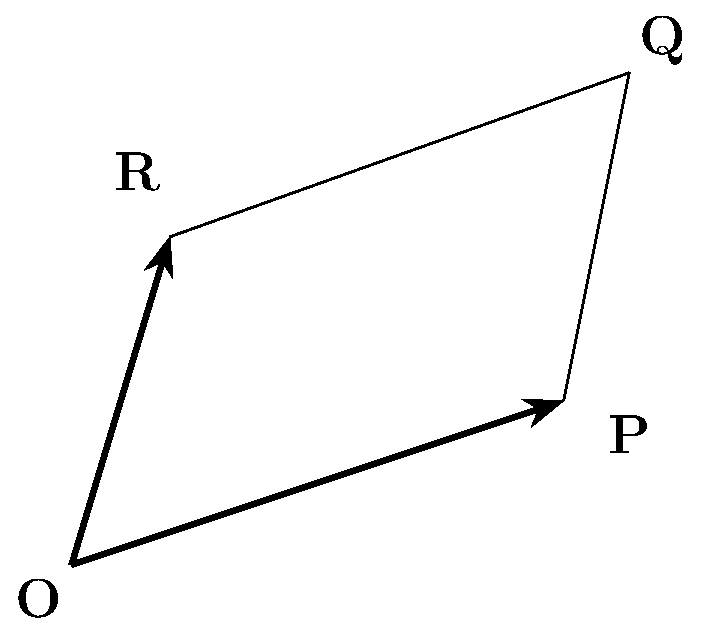
\includegraphics[width=0.2\textwidth]{figs/fig1/main} 
\end{center}
   \begin{multicols}{2}
       \begin{enumerate}
           \item $ad-bc$
           \item $ac+bd$
           \item $ad+bc$
           \item $ab-cd$
       \end{enumerate}
   \end{multicols}
   \item The solution of the ordinary differential equation $\frac{dy}{dx} + 2y = 0$ for the boundary condition , $y=5$ at $x=1$ is
   \begin{multicols}{4}
       \begin{enumerate}
           \item $y=e^{-2x}$
           \item $y=2e^{-2x}$
           \item $y=10.95e^{-2x}$
           \item $y=36.95e^{-2x}$
       \end{enumerate}
   \end{multicols}
   \item A simply supported beam is subjected to a uniformly distributed load of intensity $w$ per unit length, on half of the span from one end. The length of the span and the flexural stiffness are denoted as $l$ and $EI$, respectively. The deflection at mid-span of the beam is
   \begin{multicols}{4}
       \begin{enumerate}
           \item $\frac{5}{6144}\frac{wl^4}{EI}$
            \item $\frac{5}{768}\frac{wl^4}{EI}$
             \item $\frac{5}{384}\frac{wl^4}{EI}$
              \item $\frac{5}{192}\frac{wl^4}{EI}$
       \end{enumerate}
   \end{multicols}
   \item The sketch shows a column with a pin at the base and rollers at the top. It is subjected to an axial force $P$ and a moment $M$ at mid-height .The reaction(s) at $R$ is/are
	   \begin{center}

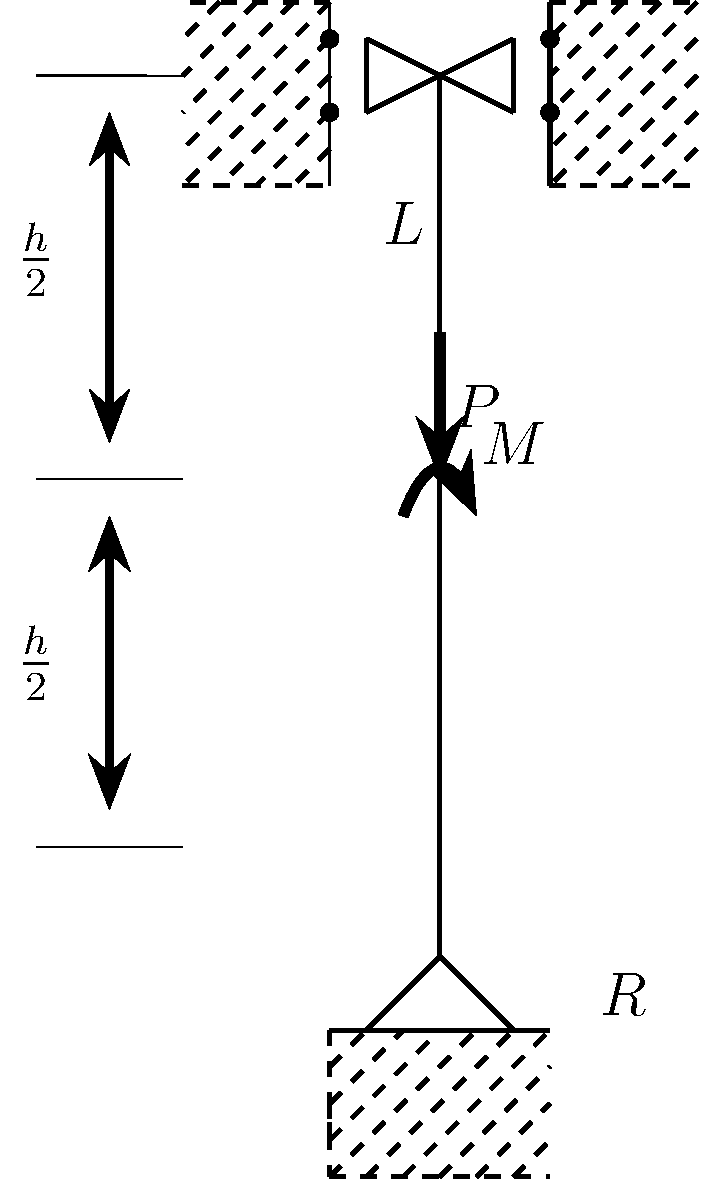
\includegraphics[width=0.15\textwidth]{figs/fig2/main} 
\end{center}
   \begin{enumerate}
       \item  vertical force equal to $P$
       \item  vertical force equal to $\frac{P}{2}$
       \item  vertical force equal to $P$ and a horizontal force equal to $\frac{M}{h}$
       \item vertical force equal to $\frac{P}{2}$ and a horizontal force equal to $\frac{M}{h}$\\
   \end{enumerate}
   \item A concrete beam prestressed with a parabolic tendon is shown in the sketch. The eccentricity of the
tendon is measured from the centroid of the cross-section. The applied prestressing force at service
is $1620$ kN. The uniformly distributed load of $45$ kN/m includes the self-weight.
\begin{center}

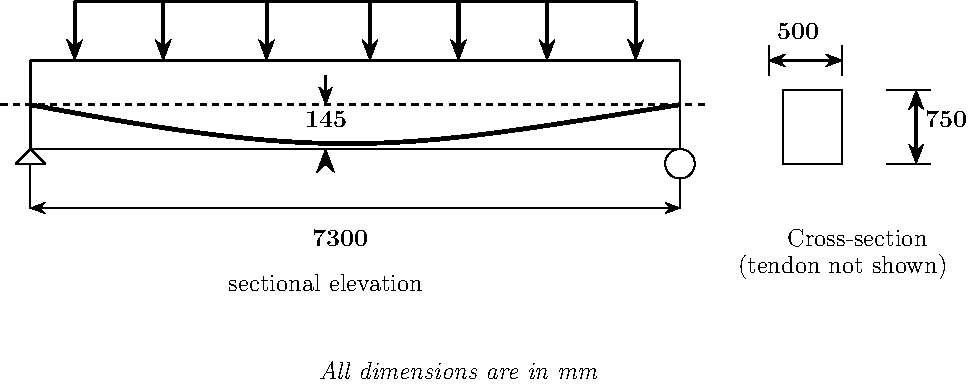
\includegraphics[width=0.8\textwidth]{figs/fig3/main} 
\end{center}
The stress $\brak{\frac{N}{mm^2}}$ in the bottom fibre at mid-span is
\begin{enumerate}
    \item tensile $2.90$
    \item compressive $2.90$
    \item tensile $4.32$
    \item compressive $4.32$\\
\end{enumerate}
\item A symmetric frame $PQR$ consists of two inclined members $PQ$ and $QR$, connected at $Q$ with a rigid joint, and hinged at $P$ and $R$. The horizontal length $PR$ is $l$. If a weight $W$ is suspended at $Q$, the bending moment at $Q$ is
\begin{multicols}{4}
    \begin{enumerate}
        \item $\frac{Wl}{2}$
         \item $\frac{Wl}{4}$
          \item $\frac{Wl}{8}$
          \item zero
    \end{enumerate}
\end{multicols}
\item Two plates are connected by fillet welds of size 10 mm and subjected to tension, as shown in the sketch. The thickness of each plate is $12$ mm. The yield stress and the ultimate tensile stress of steel are $250$ MPa and $410$ MPa, respectively. The welding is done in the workshop $\brak{\gamma_{mv} = 1.25}$. As per the Limit State Method of IS $800\colon2007$, the minimum length (rounded off to the nearest higher multiple of $5$ mm) of each weld to transmit a force $P$ equal to $270$ kN is
	\begin{center}

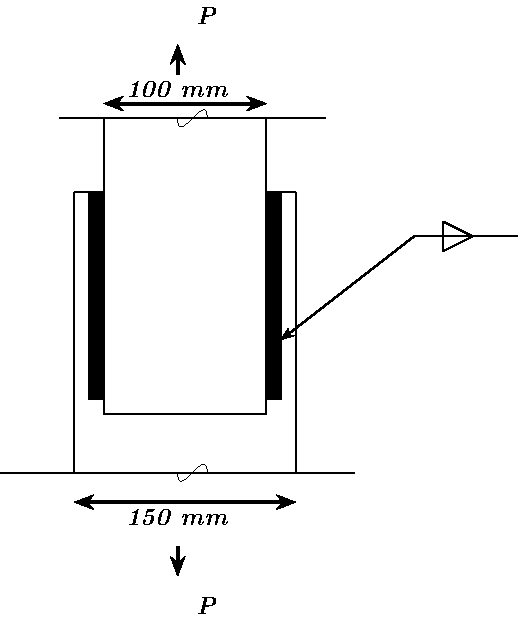
\includegraphics[width=0.5\textwidth]{figs/fig4/main} 
\end{center}
\begin{multicols}{4}
    \begin{enumerate}
        \item $100$ mm
        \item $105$ mm
        \item $110$ mm
        \item $115$ mm
    \end{enumerate}
\end{multicols}
\item Two soil specimens with identical geometric dimensions were subjected to falling head permeability tests in the laboratory under identical conditions. The fall of water head was measured after an identical time interval. The ratio of initial to final water heads for the test involving the first specimen was $1.25$. If the coefficient of permeability of the second specimen is $5$-times that of the first, the ratio of initial to final water heads in the test involving the second specimen is
\begin{multicols}{4}
    \begin{enumerate}
        \item $3.05$
        \item $3.80$
        \item $4.00$
        \item $6.25$
    \end{enumerate}
\end{multicols}
\item A layer of normally consolidated, saturated silty clay of $1$ m thickness is subjected to one dimensional consolidation under a pressure increment of $20$ kPa. The properties of the soil are:
specific gravity $= 2.7$, natural moisture content$ = 45\%$, compression index = 0.45, and
recompression index $= 0.05$. The initial average effective stress within the layer is $100$ kPa.
Assuming Terzaghis theory to be applicable, the primary consolidation settlement (rounded off to the nearest mm) is
\begin{enumerate}
    \item $2$ mm
    \item $9$ mm
    \item $14$ mm
    \item $16$ mm
\end{enumerate}
\item Steady state seepage is taking place through a soil element at $Q$,$2$ m below the ground surface immediately downstream of the
toe of an earthen dam as shown in the sketch. The water level in a piezometer installed at $P$, $500$ mm above $Q$, is at the ground surface. The water level in a piezometer installed at $R$, $500$ mm below $Q$, is $100$ mm above the ground surface. The bulk saturated unit weight of the soil is $18 kN/m^3$ and the unit weight of water is $9.81 kN/m^3$. The vertical effective stress (in kPa) at $Q$ is
\begin{center}

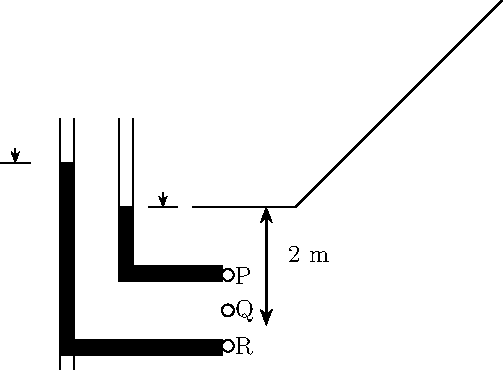
\includegraphics[width=0.5\textwidth]{figs/fig5/main} 
\end{center}
\begin{multicols}{4}
    \begin{enumerate}
        \item $14.42$
        \item $15.89$
        \item $16.38$
        \item $18.34$
    \end{enumerate}
\end{multicols}
\item The top width and the depth of flow in a triangular channel were measured as $4$ m and $1$ m, respectively. The measured velocities on the centre line at the water surface, $0.2$ m and $0.8$ m below the surface are $0.7$ m/s, $0.6$ m/s and $0.4$ m/s, respectively. Using two-point method of velocity measurement, the discharge $\brak{\text{ in  m}^3/\text{s}}$ in the channel is
\begin{multicols}{4}
    \begin{enumerate}
        \item $1.4$
        \item $1.2$
        \item $1.0$
        \item $0.8$
    \end{enumerate}
\end{multicols}
\end{enumerate}
\end{document}
